\section{Literature Review}
\subsection{Problems of Software Engineering}
Software has become an integral part of our daily lives. Certain expectations exist regarding the quality of software in terms of reliability, security and efficiency. These expectations come with challenges for the software developers across all industries.
For decades, software engineers have tried to develop methods and guides to overcome these issues. However, in 1986 Frederick Brooks published his paper `No Silver Bullet'
in which he argues that: `\ldots building software will always be hard. There is inherently no silver bullet.' \footcite[3]{brooksNoSilverBullet1987}. He based this statement on the fact that there two types of difficulties in software development: the essential and the accidental.
The essential difficulties he names are complexity, conformity, changeability and invisibility.\\
With complexity, Brooks wants to describe the inherit intricacy of software systems: `Software entities are more complex for their size than perhaps any other human construct, because no two parts are alike'.\footcite[3]{brooksNoSilverBullet1987}
This complexity makes `conceiving, describing, and testing them hard'\footcite[3]{brooksNoSilverBullet1987}.\\
The second essential difficulty Brooks names is conformity. To explain this, he compares software development to physics. Even though they are similarly complex, physics has the advantage of relying on a single set of laws or `creator'. The same cannot be said for software engineers. Brooks claims that
the complexity is `arbitrary [\ldots], forced without rhyme or reason by the many human institutions and systems to which his interfaces must conform'\footcite[4]{brooksNoSilverBullet1987}. This is due to software being perceived as `the most comfortable'\footcite[4]{brooksNoSilverBullet1987} element to change in a system.\\
Brooks explains the third issue, changeability, by comparing software to other products like cars or computers. With these types of products, changes are difficult to make once the product is released. Software however is just `pure thought-stuff, infinitely malleable.'\footcite[4]{brooksNoSilverBullet1987} Another major issue regarding changeability is
the fact that software often `survives beyond the normal life of the machine vehicle for which it is first written'\footcite[4]{brooksNoSilverBullet1987}. This means that software has to be adapted to new machines causing an extended life time of the software.\\
Invisibility is the last essential difficulty Brooks names. With this he means the difficulty to visualize software compared to other products. This not only makes the creation difficult but also `severely hinders communication among minds'\footcite[4]{brooksNoSilverBullet1987}.
According to Brooks, these issues are in `the very nature of software' \footcite[2]{brooksNoSilverBullet1987}. These difficulties are unlikely to be solved, in comparison with the accidental difficulties.\\

In contrast, the accidental difficulties arise from limitations of current languages, tools and methodologies. According to Brooks, this involves issues such as inefficient programming environments, suboptimal development processes and integration challenges which can be overcome as the industry improves its practices and technologies.\footcite[5-6]{brooksNoSilverBullet1987}
For example, the adaptation of agile methodologies, integrated development environments and continuous integration have helped to overcome some of these accidental difficulties.\\

The persistent nature of these challenges presented by Brooks have since been substantiated by further empirical research. For instance, Lehman and Ramil (2003) discussed in their paper `Software evolution—Background, theory, practice' that software systems which are left unchecked will experience a decline in quality over time.\footcite[34]{lehmanSoftwareEvolutionBackground2003}
This phenomenon is encapsulated in Lehman's laws of software evolution, which he formulated in multiple papers.  Lehman and Ramil present empirical observations supporting the notion that software quality tends to deteriorate over time\footcite[42]{lehmanSoftwareEvolutionBackground2003} - a phenomenon often described as
software decay.

\subsubsection{Software Decay}
The term software decay or erosion was empirically studied and statistically validated by Eick et al.\ in their influential paper `Does Code Decay? Assessing the Evidence from Change Management Data'(2001). They begin by stating that `software does not age or "wear out" in the conventional sense.' \footcite[1]{eickDoesCodeDecay2001}
If nothing in the environment changes, the software could run forever. However, this is almost never the case as there is a constant change in several areas, predominantly with respect to the two areas of the hard- and software environments and the requirements of the software.\footcite[1]{eickDoesCodeDecay2001}\\

The previous statement is in accordance with the first two laws of Program Evolution Dynamics formulated by Belady and Lehman (1976).
The first law states: `A system that is used undergoes continuing change until it is judged more cost effective to freeze and recreate it.'\footcite[228]{beladyModelLargeProgram1976}
Building on this, their second law declares: `The entropy of a system (its unstructuredness) increases with time, unless specific work is executed to maintain or reduce it.'\footcite[228]{beladyModelLargeProgram1976}\\

The analysis of Eick et al.\ provide empirical validation for these theoretical laws, offering `very strong evidence that code does decay.'\footcite[7]{eickDoesCodeDecay2001}
This conclusion is based on their findings that `the span of changes increases over time'\footcite[7]{eickDoesCodeDecay2001} meaning that modifications to the software tend to effect increasingly larger parts of the system as the software evolves. This growth in the span of changes indicates and potentially leads to
a breakdown in the software's modularity. Consequently the software becomes `more difficult to change than it should be,'\footcite[3]{eickDoesCodeDecay2001} measured specifically by three criteria: cost of change, time to implement change and the resulting quality of the software.\footcite[3]{eickDoesCodeDecay2001}
Therefore, the combination of theoretical insights from Lehman and Belday and empirical data from Eick et al. paints a clear picture: software decay is an inevitable consequence of ongoing evolution unless consciously and proactively managed through structured efforts such as continuous refactoring and architectural vigilance.\\

The concept of software decay aligns closely with earlier theoretical discussions by David Parnas (1994). In his influential paper `Software Aging', Parnas describes software aging as a progressive deterioration of a program's internal quality primarily due to frequent, 
inadequately documented modifications which he termed `Ignorant surgery'\footcite[280]{296790}, as well as the failure to continuously adapt the architecture to evolving needs which he called `Lack of movement'\footcite[280]{296790}.
Without this proactive maintenance and refactoring effort, Parnas argues that software inevitably reaches a state where changes become more risky, costly and error-prone\footcite[280-281]{296790}.

\subsubsection{Technical Debt}
The term `Technical Debt' was first coined by Ward Cunningham in his paper `The WyCash Portfolio Management System' (1992). This metaphor was used to describe the trade-off between a quickly implemented solution and a thought-out process. 
Using the quick solution `is like going into debt.'\footcite[2]{cunninghamWyCashPortfolioManagement1992} Cunningham argues that this debt accumulates interest if not repaid or rewritten. 
If this does not happen, Cunningham warns that `Entire engineering organizations can be brought to a stand-still under the debt load of an unconsolidated implementation'\footcite[2]{cunninghamWyCashPortfolioManagement1992}.\\

This term was further built upon and refined by the industry through white papers like `Technical Debt' by Steve McConnell (2008) or the `Technical Debt Quadrant' by Martin Fowler (2009).
McConnell differentiates between two types of technical debt: Unintentional and Intentional \footcite[3]{mcconnellManagingTechnicalDebt2017}. The first results from bad code, inexperience or unknowingly taking over a project with technical debt.
The second type is taken on purpose `to optimize for the present rather than for the future.'\footcite[3]{mcconnellManagingTechnicalDebt2017} As the first is not planned, it is difficult to avoid. The second type, however, can be managed and controlled.\\
Additionally, McConnell differentiates between different types of intentional debt. According to him, debt can be taken on a short-term or long-term basis. The short-term debt is taken on to meet a deadline or to deliver a feature. Therefore it is `taken on tactically or reactively'\footcite[3]{mcconnellManagingTechnicalDebt2017}.
The long-term debt on the other hand is more strategic and is taken on to help the team in a larger context. The difference between those two is that short-term debt `should be paid off quickly, perhaps as the first part of the next release cycle'\footcite[4]{mcconnellManagingTechnicalDebt2017}, while 
long-term debt can be carried by companies for years.\\

\begin{figure}[H]
    \centering
    \caption[]{Fowler's Technical Debt Quadrant}
    \label{fig:technicaldebtquadrant}
    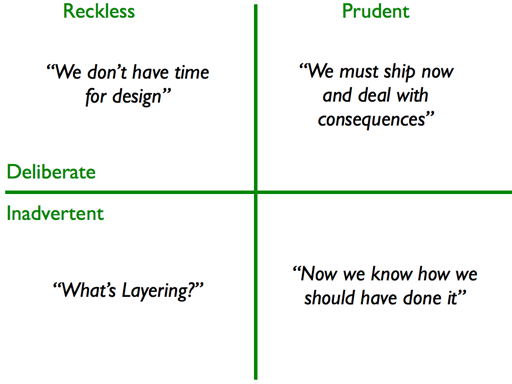
\includegraphics[width=0.5\textwidth]{techDebtQuadrant}
\end{figure}
Martin Fowler, on the other hand, warned against taking on too much deliberate debt. He argues that `Even the best teams will have debt to deal with as a project goes on - even more reason not to overload it with crummy code.'\footcite{fowlerTechnicalDebtQuadrant2009}
He created a quadrant between reckless and prudent and deliberate and inadvertent debt. For Fowler, the difference between reckless and prudent is the way the debt is taken on. Reckless debt happens without an appropriate evaluation of the consequences, risking difficulties in the future. Alternatively, prudent debt is taken on
with the trade-offs in mind and the knowledge of the future costs. Fowler differentiates between deliberate and inadvertent in a similar way to McConnell's differentiation between intentional and unintentional debt.
The various combinations of these four elements in the quadrant results in four different approaches. Reckless and deliberate would mean quick solutions without considering the long-term impact. Reckless and inadvertent results in flawed design or implementation, either carelessly or unknowingly. 
Prudent and deliberate is purposefully taking on debt to gain a short-term advantage with plans of repayment and finally prudent and inadvertent means taking on debt due to lack of knowledge or experience.\footcite{fowlerTechnicalDebtQuadrant2009}\\

In their article `Technical Debt: From Metaphor to Theory and Practice' (2012) Kruchten et al.\ criticize the concept of technical debt to be `somewhat diluted lately' \footcite[18]{kruchtenTechnicalDebtMetaphor2012}, stating that every issue in software development was called some form of debt. 
Therefore they set out to define `a theoretical foundation'\footcite[19]{kruchtenTechnicalDebtMetaphor2012} for technical debt.\\
Kruchten et al.\ state that technical debt has become more than the initial coding shortcuts and rather encompasses all kinds of internal software quality comprises.\footcite[19]{kruchtenTechnicalDebtMetaphor2012}
According to them, this includes architectural debt, `documentation and testing'\footcite[20]{kruchtenTechnicalDebtMetaphor2012} as well as requirements and infrastructure debt.
All these debt types allow engineers to better discuss the trade-offs with stakeholders and to make better decisions.\\
\\TODO: More about Kruchten and Theory?

There have been many studies providing empirical evidence for the theoretical concepts of technical debt. Highly influential studies were undertaken by Potdar and Shihab (2014) as well as by Li et al.\ (2015).\\
In their study Potdar and Shihab analyzed four large open source projects to find self-admitted technical debt as well as the likelihood of debt being removed. They found that `self-admitted technical debt exists in 2.4\% to 31\% of the files.'\footcite[1]{potdarExploratoryStudySelfAdmitted2014}
Additionally, they found that `developers with higher experience tend to introduce most of the self-admitted technical debt and that time pressures and complexity of the code do not correlate with the amount of the self-admitted technical debt.'\footcite[1]{potdarExploratoryStudySelfAdmitted2014}
They also discovered that `only between 26.3\% and 63.5\% of the self-admitted technical debt gets removed'\footcite[1]{potdarExploratoryStudySelfAdmitted2014}. This relatively low removal rate of self-admitted technical debt indicates a wider challenge:
developers recognize the issues of their implementation, but defer remediation potentially leading to a major impact on long-term maintainability.\\
Another approach to provide empirical evidence towards technical debt was taken by Li et al.\ . They conducted a systematic mapping study to `get a comprehensive understanding of the concept of "technical debt"'\footcite[194]{liSystematicMappingStudy2015}, as well as obtaining an overview of the current research in the field.
Areas of investigation included existing types of technical debt (TD), the effect of technical debt on software quality and quality attributes (QAs) as well as the limit of the technical debt metaphor.\\
They established that the `10 types of TD are requirements TD, architectural TD, design TD, code TD, test TD, build TD, documentation TD, infrastructure TD, versioning TD, and defect TD.'\footcite[215]{liSystematicMappingStudy2015}
Additionally they found that `[m]ost studies argue that TD negatively affects the maintainability [\ldots] while other QAs and sub-QAs are only mentioned in a handful of studies'\footcite[215]{liSystematicMappingStudy2015}.\\
During their studies,  Li et al. observed that the inconsistent and arbitrary use of the term `debt' among researchers and practitioners can cause confusion and hinder effective management of technical debt.\footcite[211]{liSystematicMappingStudy2015} Additionally practitioners `tend to connect any software quality issue to debt, such as code smells debt, dependency debt and usability debt.'\footcite[212]{liSystematicMappingStudy2015}
This indicates an inflationary use of the term, which is important to keep in mind when speaking about technical debt.\\

The implications these studies have for the software industry are significant. They show that software decay and technical debt are tangible and measurable in real world software projects.
In their paper `Software complexity and maintenance costs' (1993) Banker et al. empirically demonstrated that `software maintenance costs are significantly affected by the levels of existing software complexity.' \footcite[12]{bankerSoftwareComplexityMaintenance1993}
This finding emphasizes the important of proactively managing the software quality and addressing debt early in the project lifecycle, to keep the complexity and therefore cost to a minimum.\\
To address these effects, practitioners strongly recommend refactoring. Fowler argued in his book `Refactoring: Improving the Design of Existing Code' (2019)
that `[w]ithout refactoring, the internal design - the architecture - of software tend to decay.'\footcite[58]{fowlerRefactoringImprovingDesign2019}
To prevent this, he suggests `[r]egular refactoring [to] help[s] keep the code in shape'\footcite[58]{fowlerRefactoringImprovingDesign2019}.\\
To prevent long-term issues, practitioners recommend actively managing technical debt through refactoring, tracking and other strategies 
that integrate debt management into the software development process.\\

\subsubsection{Conclusion}

This chapter has outlined the foundational challenges inherent to software engineering and introduced two critical concepts: software decay and technical debt.
Drawing on Frederick Brooks' distinction between essential and accidental difficulties, it becomes evident that complexity, changeability and lack of uniformity are deeply rooted in the nature of software itself and cannot be fully resolved.
These enduring challenges are the foundation of the concepts of software decay and technical debt.\\

Software Decay refers to the gradual degradation of a software system's internal quality, leading to reduced maintainability, increased complexity and higher change effort. This is a natural outcome of continuous system evolution in a response to changing requirements and environments.
As shown through empirical work of Eick et al. and the theoretical contributions of Lehman and Parnas, software that is not actively maintained becomes harder to main, less modular and more fragile, making decay a systematic and long-term threat to software sustainability.\\

On the other hand, technical debt captures the intentional or unintentional compromises made during software development that create short-term advantages but lead to long-term costs. Originating as a metaphor, it has since evolved into a structured framework for describing, architectural design, code or process-related liabilities.
While software decay can be seen as a developing property of ongoing change, technical debt often originates from conscious decisions. Whether this is due to deadlines, insufficient knowledge or lack of resources, it manifests through debt like code quality deterioration, architectural erosion or insufficient testing.\\

Importantly, technical debt and software decay are closely related: unmanaged technical debt accelerates software decay, while software decay can lead to the accumulation of technical debt. Empirical studies from Potdar, Li and Banker confirm the measurable impact of these phenomenon on maintenance costs, defect rates and overall system quality.\\

To effectively manage these issues, the software industry has developed strategies that go beyond reactive maintenance. Structured, proactive practices such as continuous refactoring, rigorous quality assurance, technical debt management and automated testing are essential to prevent the accumulation of debt and decay.
Based on these foundations, the next chapter will explore concrete mitigation strategies in commercial environments providing a comprehensive overview of the most common strategies, techniques and frameworks used in the industry to address technical debt and software decay.\\



\subsection{Mitigation Strategies in Commercial Environments}
Technical debt and software decay have been recognized as significant challenges in the software industry. They can lead to 
increased maintenance costs, reduced software quality and decreased developer productivity, overall resulting in a more expensive and less competitive product.
With these challenges in mind, practitioners and researchers have developed a variety of strategies which manage, prevent and mitigate technical debt.
This section will provide an overview of the most common strategies, techniques and frameworks used in commercial environments to address technical debt.\\

\subsubsection{High-Level Mitigation Strategies}
To efficiently mitigate software decay and technical debt, proactive management strategies are essential. These strategies aim to prevent the accumulation of 
debt and address software entropy and decay directly by integrating quality assurance into everyday development process.
Such strategies include Agile methodologies like Scrum or \ac{XP} as well as technical practices
such as \ac{CI/CD}. These practices are designed to embed ongoing maintenance and quality assurance into routine workflows, thus combating software entropy at its core.\\
Agile methods emphasize frequent iterations, close collaboration between developers and stakeholders as well as continuous refactoring to prevent the
gradual degradation of software quality and mitigation of software decay.\\
Similarly, \ac{CI/CD} introduces rigorous automation, rapid feedback loops and early detection of defects to proactively control both technical debt accumulation
and broader software quality decay. Collectively, these methodologies create a culture of continuous improvement, adaptability and quality assurance, 
ensuring software maintainability and long-term project sustainability.\\

\paragraph{Agile Methodologies}
In their paper `Technical Debt Management in Agile Software Development: A Systematic Mapping Study' (2024)\footcite{leiteTechnicalDebtManagement2024} Leite et al.
investigated how agile methods can be used to manage technical debt. They found that `\ldots Scrum and Extreme Programming are the most utilized methodologies 
for managing technical debt.'\footcite[318]{leiteTechnicalDebtManagement2024} While this study focuses explicitly on technical debt, both Scrum and \ac{XP}
also inherently address the broader issue of software decay by encouraging proactive quality management and continuous improvement practices.\\
Scrum was first presented by Ken Schwaber in his paper `SCRUM Development Process' (1997)\footcite{schwaberSCRUMDevelopmentProcess1997}. 
It has since become one of the most popular agile frameworks in the software industry. Scrum explicitly manages software quality and technical debt through iterative cycles called sprints.
After each sprint, the team reflects on their work, identifies quality issues, technical debt and potential decay indicators and plans improvements in
retrospectives. Leite et al. found that the most used artifacts for identifying technical debt in Scrum are the Sprint and Product Backlog.\footcite[315]{leiteTechnicalDebtManagement2024}
By explicitly managing these items with their workflow, teams effectively reduce both debt and software entropy, improving overall software maintainability.\\

\ac{XP} was first introduced by Kent Beck in his influential book `Extreme Programming Explained' (1999)\footcite{beckExtremeProgrammingExplained1999}.
It explicitly integrates practices to enhance software quality and directly prevent software decay.
\ac{XP} practices such as pair programming, \ac{TDD}, \ac{CI} and continuous refactoring help maintain high software quality, thus preventing both debt accumulation
and broader software entropy.
Pair programming prevents decay by securing higher-quality code through collaborative review and knowledge sharing between developers.
\ac{CI} provides regular, frequent code integration, significantly reducing integration complexity and associated decay risks.
\ac{TDD} establishes robust test coverage, catching defects early and preventing quality erosion.
The effectiveness of refactoring, a cornerstone XP practice, has been proven empirically. For example, in their case study (2008) Moser et al.
demonstrated that refactoring explicitly `prevents an explosion of complexity'\footcite[262]{moserCaseStudyImpact2008}
and promotes simpler, easier-to-maintain designs.
They found it drove developers toward simpler designs, reducing complexity, coupling, and long-term maintenance issues thereby directly counteracting software decay.\footcite[262]{moserCaseStudyImpact2008}
Beck argues that \ac{XP}'s incremental, continuous quality practices consistently maintain software quality and adaptability throughout development, directly addressing both debt and broader software decay.\\
On the whole, agile methodologies, particularly Scrum and \ac{XP}, systematically manage technical debt and proactively prevent software decay by fostering continuous improvement, structured quality management and adaptability.
Complementing these Agile practices, the adoption of automated \ac{CI/CD} pipelines further enhances the proactive management of both technical debt
and broader software decay through rigorous quality control and systematic automation.\\

\paragraph{Continuous Integration/Continuous Deployment}
\ac{CI} was first introduced by Beck in the context of \ac{XP} and later refined by Martin Fowler in his influential article `Continuous Integration'\footcite{fowlerContinuousIntegration2006}.
Fowler describes \ac{CI} as not only the frequent, automated integration of code into the main repository but also the systematic automation of building and testing process.
According to Fowler, `Self-testing code is so important to Continuous Integration that it is a necessary prerequisite.'\footcite{fowlerContinuousIntegration2006}.
Furthermore, another critical prerequisite is `that they can correctly build the code,'\footcite{fowlerContinuousIntegration2006} thus guaranteeing that code changes consistently
integrate without issues.\\

To further prevent technical debt and broader software decay, quality analysis tools such as static code analyzers like SonarQube or DeepSource are frequently integrated into
\ac{CI} pipelines. These tools often provide a metric to evaluate technical debt which is calculated based on the effort in minutes to fix the found maintainability issues.\footcite{sonarqubeUnderstandingMeasuresMetrics2025}
In their paper `Technical Debt Measurement during Software Development using Sonarqube: Literature Review and a Case Study' (2021)\footcite{murilloTechnicalDebtMeasurement2021}
Murillo et al. found that SonarQube is a useful tool for early debt detection. The estimated remediation effort metric allows for a good debt management prioritization.\footcite[5]{murilloTechnicalDebtMeasurement2021}
However during their research they noticed if they changed SonarQubes default rules by just 26 rules, the technical debt effort would increase from
1 hours and 50 minutes to 11 hours.\footcite[4]{murilloTechnicalDebtMeasurement2021} This issue, together with the fact that SonarQube can only detect code related debt and not other debt such as
infrastructure or requirements debt, makes these tools useful but not a complete solution.\\

\ac{CD}, introduced by Jez Humble and David Farley in their foundational book `Continuous Delivery: Reliable Software Releases through Build, Test, and Deployment Automation' (2010)
extends \ac{CI} by automating the entire software release pipeline. \ac{CD} ensures that the software is always in a releasable state.
According to Humble and Farley, implementing a functional \ac{CD} pipeline `creates a release process that is repeatable, reliable, and predictable'\footcite[17]{humbleContinuousDeliveryReliable2010}.
Beyond predictability, additional significant benefits include team empowerment, deployment flexibility and substantial error reduction.
Specially, \ac{CD} effectively reduces errors, particularly those introduced by poor configuration management, including problematic areas such as
`configuration files, scripts to create databases and their schemas, build scripts, test harnesses, even development environments and operating system configurations'\footcite[19]{humbleContinuousDeliveryReliable2010}.\\

\subsubsection{Code-Level Practices for Preventing Decay}
On the code level, a variety of practices can be used to prevent software decay and technical debt. The two major practices have been previously introduced: continuous refactoring and maintaining software quality.\\
The benefits of refactoring have been demonstrated in the previous section. However, deeper empirical research illustrates the impacts and challenges in a commercial environment.
Kim et al. (2014) observe in their paper `An empirical study of refactoring challenges and benefits at Microsoft' that `[d]evelopers perceive that refactoring involves substantial cost and risks'\footcite[17]{kimEmpiricalStudyRefactoringChallenges2014}.
Additionally they describe the benefits refactoring brings as `multidimensional'\footcite[17]{kimEmpiricalStudyRefactoringChallenges2014}. Furthermore it is not consistent across different metrics, leading to their recommendation of a tool to monitor the impact of refactoring across these metrics\footcite[17]{kimEmpiricalStudyRefactoringChallenges2014}.
Similarly, Tempero et al. (2017) established certain barriers to refactoring in their study `Barriers to refactoring'. They found that at least 40\% of the developers in their study would not refactor classes, even though they thought it would be beneficial. \footcite[60]{temperoBarriersRefactoring2017}\\
Tempero et al. claims the reasons were `lack of resources, of information identifying consequences, of certainty regarding risk, and of support from management'\footcite[60]{temperoBarriersRefactoring2017} even though developers did not state a lack of refactoring tools as a reason.
To eliminate these barriers, Tempore et al. suggest refactoring should be goal-oriented instead of operations-oriented and a better quantification of the benefits refactoring should bring to better reach a decision.\footcite[61]{temperoBarriersRefactoring2017}\\
Both studies show that the theoretical benefits of refactoring are not always directly translated into the industry. Developers often perceive refactoring as risky and costly, even though they are aware of the benefits.\\

\ac{TDD} is another code-level practice previously introduced. It was first formally described by Kent Beck in his book
`Test Driven Development: By Example' (2002) in which he argues that writing tests before the implementation
encourages cleaner code and gives developers the confidence to tackle complex problems.\footcite[pp. 8-9]{beckTestdrivenDevelopmentExample2002}
This practice promotes modularity, testability and clean design, key characteristics in preventing software decay. By focusing solely on code
that fulfills predefined tests, developers are guided toward creating small and focused code, which is loosely coupled. These qualities make systems
easier to maintain and refactor, directly counteracting long-term degradation.
Multiple studies have confirmed the quality-enhancing effects of \ac{TDD}.
In an empirical study, Mäkinen and Münch (2014) found that  TDD most commonly led to a reduction in defects and increased maintainability, 
although its effect on overall software quality was more limited.\footcite[13]{inproceedings}
Importantly, they note that TDD significantly improves test coverage, a key factor in preventing unintentional decay.
These gains, however, were accompanied by higher development effort.\footcite[13]{inproceedings}\\
This is consistent with the case study by Bhat and Nagappan (2006), who reported a 15-35\% increase in development time when using \ac{TDD}.\footcite[361]{bhatEvaluatingEfficacyTestdriven2006a}
However they also observed that `the resulting quality was higher than teams that adopted a non-TDD approach by an order of at least two times.'\footcite[361]{bhatEvaluatingEfficacyTestdriven2006a}
Similarly, Bhadauria et al. (2020) confirm TDD’s positive effect on code quality and defect reduction.
Interestingly, their study found that for less experienced developers, TDD did not lead to increased development time, and was associated with higher developer satisfaction.\footcite[1058]{bhadauriaPerformanceOutcomesTestDriven2020}\\
These findings indicate that TDD can significantly improve code quality and maintainability two critical factors in preventing software decay.
However, the trade-off in development effort and time must be carefully considered, which may explain TDD's limited adoption in the industry.\\

\subsubsection{Architectural Strategies for Long-Term Quality}
In addition to code-level practices, the maintenance of the software architecture is essential for preventing software decay and architectural-level technical debt. 
Architecture erosion, characterized by increasing divergence from the intended design due to continuous modifications and changing requirements,
significantly impacts maintainability and introduces substantial technical debt.\footcite[1]{desilvaControllingSoftwareArchitecture2012}
One common strategy to mitigate these risks,  is architecture conformance checking, a process ensuring code changes comply with predefined design rules.
De Silva and Balasubramaniam (2012) emphasize that proper documentation, dependency analysis and compliance monitoring are critical prerequisites for
effectively employing this strategy.\footcite[135]{desilvaControllingSoftwareArchitecture2012}\\
Beyond mere conformance, teams must also embrace managed architectural evolution, adapting architectures systematically rather than reactively. Such evolution
should actively balance new requirements with long-term sustainability to avoid uncontrolled erosion.\footcite[34]{liUnderstandingSoftwareArchitecture2022}
A key component in this proactive approach is managing the architectural technical debt. These structural design decisions could impact future adaptability if not
carefully controlled. Besker et al. (2016) suggest a framework to systematically identify, analyze and address architectural debt to preserve structural integrity.\footcite[11]{beskerManagingArchitecturalTechnical2018}\\
Nevertheless, when architectural decay becomes substantial, teams face critical decisions between incremental refactoring and radical redesigns.
Nord et al. (2012) highlight that systematic impact analysis, guided by explicit architectural metrics, is crucial for making informed decisions on when substantial 
redesign becomes necessary to substantially restore software quality.\footcite[99]{nordSearchMetricManaging2012}\\
Practical tooling, such as automated architectural monitoring and recovery solutions, plays a significant supportive role in these efforts. 
The detailed application and empirical evidence of such tools issue discussed thoroughly in the subsequent section on Tool Support for Continuous Quality Assurance.\\

In summary, proactively maintaining software architecture is essential for mitigating long-term software decay. Architecture conformance checking 
prevents the inadvertent erosion by ensuring adherence to established design principles. Managed architectural evolution further ensures that the architecture
can sustainably adapt to changing requirements without introducing uncontrolled structural degradation. Moreover, explicitly recognizing and managing architectural
technical debt enables targeted interventions before significant decays occurs. Ultimately, strategic decisions on refactoring versus comprehensive redesign should be 
guided by systematic architectural analysis, metrics and empirical evaluations to ensure long-term maintainability and quality.

\subsubsection{Process and Organizational Measures}
Organizational and process-oriented practices form the third pillar in combating software decay.
One crucial practice is the management of technical debt. Many companies track technical debt items like outdated modules, quick fixes or known architectural shortcomings.
This can be done through issue trackers or backlogs to allow for structured approach and time allocation to address them regularly.
An industry-wide survey conducted by Ramač et al. (2021) found that 47\% `had some practical experience with TD identification and/or management'\footcite[40]{ramacPrevalenceCommonCauses2021}.
By visualizing and tracking technical debt, teams can prioritize and address debt items systematically, preventing their accumulation and broader software decay.
Ramač et al. also found that the most common cause for technical debt was time pressure caused by deadlines\footcite[40]{ramacPrevalenceCommonCauses2021} and the `single most cited effect of TD is delivery delay.'\footcite[40]{ramacPrevalenceCommonCauses2021}
This indicates that time pressure is not only a cause of technical debt but also a consequence, leading to a vicious cycle of debt accumulation and delivery delays. To break this cycle, a balance of new development and maintenance is crucial to prevent a border software decay.
This is promoted by agile methodologies through the principle of continuous improvement, practices like including refactoring in their definition of done or allowing dedicated maintenance sprints.

Another important practice is conducting regular code reviews as part of the development workflow. This practice dates back to 1976 when Michael Fagan reviewed the benefits of peer code inspections.\footcite[183]{faganDesignCodeInspections1976}
He found that `inspections increase productivity and improve final program quality.'\footcite[205]{faganDesignCodeInspections1976}
Since then, code reviews have become more lightweight compared to the inspection proposed by Fagan, increasing participation. By removing in-person meetings and reviewer checklists, code reviews have become a standard practice in software development and usually occur before code is merged into the main repository.
McIntosh et al. (2016) investigated the impact of code reviews on software quality by comparing the review coverage, participation and expertise of the reviewer against the post-release defects.\footcite[6]{mcintoshEmpiricalStudyImpact2016}
They found that coverage, while important, is not the only factor that influences the post-release defects.\footcite[39]{mcintoshEmpiricalStudyImpact2016}
They state that `review participation should be considered when making integration decisions.'\footcite[39]{mcintoshEmpiricalStudyImpact2016}
Additionally, they recommend that if an expert in the matter is not available for the original code, they should be included in the review process to prevent defects.\footcite[39]{mcintoshEmpiricalStudyImpact2016}

In conclusion, structured approach to managing technical debt and preventing software decay is crucial to maintain software quality and long-term project sustainability.
Process-integrated practices like code reviews, explicit technical debt control and a culture of continuous refactoring create an environment that proactively manages software decay and technical debt.

\subsubsection{Tool Support for Continuous Quality Assurance}
To further support the proactive management of software decay, technical debt and the overall code health over time, a variety of tools have established themselves in the industry.
Automated quality assurance tools are often integrated into modern development processes. A common approach, as previously mentioned, is the use of \ac{CI} pipelines. These can be used in combination with quality gates which use static code analysis to block additions to the code base that do not meet the quality standards e.g. a 
certain code coverage, complexity or maintainability threshold. This allows developers to catch issues early and rectify them before they are introduced into the code base . While the concept of quality gates is not new, the automation of these gates have recently been investigated by Uzunova et al. (2024).
They found that these gates can serve as a check point to assess software metrics like code coverage, bug density or compliance with coding standards. \footcite[8]{uzunovaQualityGatesSoftware2024}
To allow for this kind of automation, they suggest tools like SonarQube, Sigrid or Maverix.ai. These tools provide real-time feedback allowing for an enforcement of quality criteria.\footcite[8]{uzunovaQualityGatesSoftware2024}\\
Utilizing this approach enables developers to catch issues early and prevent the introduction of technical debt and software decay into the codebase.\\

As discussed in a previous section, ensuring that changes do not divert from the original architecture design is crucial to prevent the erosion of the architecture.
To support this, tools have been developed to automatically detect architecture violations. These tools are able to collect information about the architecture from the source code
and compare it to the proposed architecture.\footcite[6]{thomasStaticDynamicArchitecture2017} In their case study 
`Evaluating an Architecture Conformance Monitoring Solution' (2016), Caracciolo et al. investigated three different tools to detect architecture violations:
SonarQube, Sonargraph and TeamCity\footcite[43]{caraccioloEvaluatingArchitectureConformance2016}. They concluded that their approach 
`can be applied in an industrial context.'\footcite[44]{caraccioloEvaluatingArchitectureConformance2016}
They furthermore argue that the tools can be conveniently added to a dashboard, allowing for a short feedback loop as well as proactive management of architectural violations.\footcite[44]{caraccioloEvaluatingArchitectureConformance2016}
These benefits can be seen in their case study, where they observed that the overall violations decreased from 606 to 600 in an 18 year old system with one million lines of code\footcite[43]{caraccioloEvaluatingArchitectureConformance2016}.\\

Numerous empirical studies show the effectiveness of these tools. In their paper `Empirical investigation of the influence of continuous integration bad practices on software quality' (2022),
Silva and Bezerra found that `CI can improve software quality, especially about cohesion.'\footcite[4]{silvaEmpiricalInvestigationInfluence2022} However they also observed the impact
of bad practices in the implementation of CI. They found that the quality levels were incorrectly set and the standard configuration tools were used instead of 
adjusting them to the project needs, which overall harmed the software quality indicators. \footcite[4]{silvaEmpiricalInvestigationInfluence2022}
This indicates that, for the tools to be effective, they need to be correctly configured and adjusted to the project needs.\\

\subsubsection{Synthesis of Commercial Mitigation Strategies}
Effectively managing software decay and technical debt requires a balanced combination of technical, architectural and organizational strategies.
At the highest level, Agile methodologies and \ac{CI/CD} frameworks foster proactive maintenance cultures, reducing entropy through incremental improvement
and automated quality assurance. On the code level, disciplined practices such as continuous refactoring and \ac{TDD} have empirically demonstrated their effectiveness
in maintaining modularity, testability and reducing technical debt - with the downside of a higher development effort. Architectural strategies complement these
by ensuring structural integrity through systematic conformance checks, managed evolution and explicit handling of architectural technical debt, especially as
the scale or requirements of projects evolve.

Organizational measures such as technical debt tracking, dedicated maintenance cycles and structured code reviews provide essential process-level support,
enabling teams to systematically prioritize and address decay risks before they escalate. Finally, the strategic use of modern quality-assurance tools, integrated
into \ac{CI} pipelines and architectural monitoring systems, ensures continuous, automated and actionable feedback, thereby enabling developers to maintain
software quality proactively. Ultimately, integrating these diverse practices into a combined quality culture is vital for sustainable software development,
reduced maintenance costs and the long-term viability of software products.\\


\subsection{Unique Constraints in Military Software Development}
\subsubsection{Introduction to Military Software Context}
Software development for military significantly differs from commercial software due to unique demands for high reliability, rigorous security, and extended system lifecycles.
The \ac{NRC} book `Reliability Growth: Enhancing Defense System Reliability' (2015) highlights the difference between commercial and military software development.
According to them there are three main differences. The first is about the `sheer size and complexity of defense systems'\footcite[31]{nrc2015defense}.
These systems often have a vast amount of individual elements that need to work together, that also evolve over time, as the architecture changes between the different stages of 
the lifecycle.\footcite[32]{nrc2015defense} In addition, the \ac{NRC} highlights the fact that new systems have to interact with legacy systems, which can be a challenge
due to the different technologies and architectures used.\footcite[32]{nrc2015defense}
The second difference are the different perspectives of the actors involved. Unlike in the commercial environment, where it is usually only the project manager 
that controls the vision and the goals of the project, in the military environment there are multiple stakeholders with different goals in mind.\footcite[32]{nrc2015defense}
even though the book specially talks about the American military, the same can be said for the German military.
The third difference the authors name are the concerns of risk. In the commercial environment, the manufacturer has a self interest in the product being successful and reliable.
In the military environment however, the government is the customer and often holds the most risk, as they are the ones that have to use the product in the end.
The NRC claims that this result in `the system developers do not have a strong incentive to address reliability goals early in the acquisition process'\footcite[33]{nrc2015defense}.
especially because the downstream benefits are not quantifiable for the developers.\footcite[33]{nrc2015defense}\\
In her presentation on `A perspective on military software needs' Heidi Shyu highlights additional challenges in military software development.
She argues that in addition to the complex setting, there are often a multitude of contractors working together, having to interoperate in real time with each other.\footcite[11]{shyu2017military}
Often these projects have a lifecycle of decades compared to the commercial software lifecycle of a few years.\footcite[14]{shyu2017military}
Due to these long lifecycles, the software needs to developed so it can be easily maintained and updated, while still working with legacy systems
which often have very specific requirements.\footcite[14]{shyu2017military}
Therefore, Heidi Shyu claims, the architecture has to last for decades, however soft- and hardware changes much faster, often resulting in a patchwork of quick fixes.\footcite[15]{shyu2017military}
She names examples for needed software solutions like a flexible architecture which allows for easy updates and addition, self-testing modular code and intuitive, easy to use interfaces.\footcite[17]{shyu2017military}\\

In summary, these challenges in military software development are unique to the industry. The vast size and complexity of defense systems,
their long lifecycles and the multitude of stakeholders involved create a complex environment that requires specialized strategies to manage software decay and technical debt effectively.

\subsubsection{Regulatory and Procurement Constraints in the Bundeswehr}
The procurement and regulatory environment significantly shapes military software development in the German Armed Forces (Bundeswehr). Unlike commercial settings,
Bundeswehr software projects are tightly governed by formalized frameworks, rigorous approval processes and comprehensive regulations designed primarily to ensure 
accountability, security, and reliability. However, these structures can inadvertently limit agility, prolong software updates and contribute significantly to software decay
and technical debt over time.\\

Bundeswehr software utilizes the `V-Modell XT Bw' as the project lifecycle model. It is a customized variant of the standard V-Modell XT, specifically tailored to Bundeswehr needs and closely integrated with the 
Bundeswehr's overarching procurement framework, \ac{CPM}.
The V-Modell XT Bw is a comprehensive framework that encompasses the planning and execution of software projects in the Bundeswehr.\footcite[6]{bundeswehrVModellXTBw}
It includes detailed guidelines for all parts of the software development process, from roles and requirements engineering to \ac{QA} and product quality.\footcite[pp. 20-21]{bundeswehrVModellXTBw}
However, due to its rigid and sequential nature, the waterfall-based V-Modell XT Bw is known to limit flexibility, making iterative adjustments and agile methodologies challenging to implement.\\

The procurement procedures of the Bundeswehr are outlined by the aforementioned \ac{CPM} which was revised in 2012 after a commission in 2010 found that: 
`Die Streitkräfte erhalten ihre geforderte Ausrüstung zumeist weder im erforderlichen Zeit- noch im geplanten Kostenrahmen.'\footcite[36]{strukturkommissionderbundeswehrBerichtStrukturkommissionBundeswehr2010}.
Due to these problems, the revised \ac{CPM} has an increased focus on upfront requirement definition and comprehensive risk assessments. This creates long lead times
for approval and makes quick technological changes difficult to realize.
In addition, the \ac{EVB-IT}, the standardized contracts for government IT solutions, hinders agile development. This is according to Holger Schröder in an article  from 2022
where he claims that multiple different contract blueprints would have to be combined to allow for an agile development project.\footcite{schroederUngeeignetFuerAgile2022}

Collectively, all these requirements and procurement constraints strongly influence software development practices. Control and predictability are prioritized, making
a iterative and agile framework difficult to use. While these procedures promote accountability and reduce risk, they can severely limit a system's ability to evolve over time, thereby fostering conditions under which software decay and technical debt accumulate. 
Adding to this complexity are strong security and compliance requirements, which are discussed in the following subsection.

\subsubsection{Security and Compliance Requirements}
Military software must meet stringent security and compliance standards beyond the usual commercial requirements. Due to the sensitive nature of military operations and data,
the software must adhere to both national and NATO standards. These strict requirements create severe difficulties 
towards the lifecycle of the product, the software architecture and maintenance practices. These constrains accelerate the accumulation of technical debt and software decay.\\

Like all federal agencies in Germany, the Bundeswehr must adhere to the \ac{BSI} guidelines for IT security called IT-Grundschutz\footcite{bundesamtfuersicherheitinderinformationstechnikBSIFAQ}. Through several standards it defines a comprehensive security framework
that includes technical, personnel and infrastructural security measures. Compliance with these standards involve extensive documentation, risk management process and regular audits. This increases the complexity and effort required for ongoing software maintenance and updates.\footcite{bundesamtfuersicherheitinderinformationstechnikBSIStandards}\\

In addition to the national regulations, Bundeswehr software systems must comply with the NATO security standards. These guidelines establish requirements towards handling of classified data, encryption standards and security clearance of personnel.
An example would be the NATO Security Policy (C-M(2002)49) which dictates the handling of NATO-classified information, constraining software flexibility and maintenance practices\footcite[Enclosure B, pp. 1–3; Enclosure F, pp. 1–2]{NATO2002SecurityPolicy}. 
Compliance with NATO standards mandates extensive security accreditation procedures, detailed documentation and comprehensive vetting of software and hardware systems.
These processes slow down software development cycles and restrict flexibility due to the necessity of re-certifying software after significant changes.

Furthermore the Bundeswehr adheres to national classification rules, such as \ac{VS-NFD}. Systems classified under \ac{VS-NFD} require access control, encrypted communications, dedicated network infrastructure and periodic security accreditation.\footcite[see Part 2, pp. 1–3; Part 3, pp. 1–6]{BMI2010VSNFD}
Developers and system administrators must adhere to strict usage guidelines, which dictate the permissible software, hardware and methods of data handling.\footcite[Part 3, No. 3.1–3.7, pp. 1–5]{BMI2010VSNFD} Compliance significantly restricts the usage of modern technologies such as cloud services or external software libraries, unless explicitly cleared\footcite[Part 3, No. 3.4.1–3.4.5, pp. 4–5]{BMI2010VSNFD}, 
which can be seen in the example of Genua’s secure remote working solution, which complies with both VS-NfD and NATO security requirements while offering functionality typically restricted in classified environments.\footcite{Genua2023VSNFD}

Although essential for operational security, these security and compliance requirements markedly constrain software adaptability and agility. 
Extensive documentation, mandatory security certifications, and regular audits mandated by national and international regulations considerably increase the maintenance workload and complexity. 
Consequently, prolonged approval processes and heightened architectural complexity often accelerate software decay and technical debt accumulation, complicating extensive refactoring or proactive architectural evolution.

In summary, security and compliance requirements play a pivotal role in shaping Bundeswehr software development practices, significantly influencing architecture design, 
maintenance methodologies, and lifecycle management. While crucial for safeguarding operational security and classified information, these rigorous standards often inhibit software adaptability and innovation, exacerbating the challenges of software decay and technical debt inherent in military software systems.

\subsubsection{Legacy Systems and Extended Lifecycles}
Legacy systems and extended lifecycles impose particularly significant constraints within military software projects, especially within the Bundeswehr. 
Unlike commercial software, which typically operates for a limited period, military systems frequently remain operational for decades due to high investment costs, complexity, and risk aversion to adopting new technologies. Such prolonged operational 
lifespans inevitably contribute to technical debt accumulation and progressive software decay, significantly complicating maintenance and increasing lifecycle costs.

A prominent example of these challenges emerged with the Bundeswehr's logistics and support IT systems at the turn of the century. According to Sebastian Stein's 2011 blog entry,
 the Bundeswehr managed around 1,200 distinct outsourced IT systems, creating a highly fragmented and inefficient infrastructure.\footcite{steinBusinessProcessManagement2011} To address this issue, the Bundeswehr initiated the \ac{SASPF} program, consolidating procurement, accounting, 
 and logistics systems into a single, integrated SAP-based solution. However, standard SAP software initially met only around 70\% of the Bundeswehr's unique operational requirements, necessitating extensive custom development and temporary workarounds.\footcite{steinBusinessProcessManagement2011} These integrations were further 
 complicated by stringent regulatory requirements, diverse stakeholder interests, and interoperability challenges with outdated technologies. Consequently, significant technical debt and complexity accumulated, extending the modernization effort well over a decade and clearly demonstrating the severe maintenance implications of legacy systems.\footcite{steinBusinessProcessManagement2011}

Another illustrative case within the Bundeswehr is the Luftwaffe's Tornado fighter jet program. Development began in 1981, and the aircraft entered operational service in 1992. Today, approximately 80 Tornado jets remain operational, with plans for 
replacement only by 2030 resulting in a nearly 50-year lifecycle.\footcite{skibaTornado50Jahre2024} Continuous software updates have been crucial throughout this extensive period, including notable upgrades like the integration of the RecceLite reconnaissance system in 2009. However, 
each update has progressively become more complex and costly due to aging hardware, software architecture limitations, and stringent compliance demands. This incremental layering of software modifications directly contributes to accelerated software decay, increasing the difficulty and expense of maintaining operational effectiveness.

Comparable challenges are prevalent among international NATO allies as well. A notable example was highlighted by Kynan Carver (2022), describing how the U.S. \ac{DOD} continued operating critical strategic systems reliant on severely outdated technologies, 
including 8-inch floppy disks, until the late 2010s.\footcite{carverTechnicalDebtCybersecurity2022} Carver emphasizes that maintaining these aging software infrastructures consumes significant financial and operational resources, limiting investment in innovation and proactive modernization strategies.\footcite{carverTechnicalDebtCybersecurity2022}

In conclusion, effectively managing technical debt and mitigating software decay within military systems requires strategic, long-term investments, proactive modernization plans, and an explicit focus on maintainability. Addressing the unique challenges posed by legacy 
systems and extended lifecycles is thus crucial for sustaining operational capability and flexibility within an increasingly dynamic military technology environment.

\subsubsection{Conclusion}
Military software development is fundamentally shaped by demands that are far beyond those of the commercial environments. The need for extreme reliable, long lasting systems while having strict classification regimes and multi-layered stakeholder requirements creates a highly regulated and risk-shy context.
These characteristics collectively contribute to a development landscape where software decay and technical debt are not merely byproducts of poor practices but structural risks embedded within the system's lifecycle.\\

As shown throughout this section, four constraint areas amplify these challenges. First the inherit complexity and longevity of military systems, often designed to operate for decades, create pressure to extend the viability of aging platforms.
Secondly the rigid procurement and development frameworks, such as the V-Modell XT Bw and the \ac{CPM} process, prioritize upfront control and traceability over agility, hindering adaptive or incremental development practices.
Third, extensive national and NATO security requirements impose detailed compliance burdens, restricting the use of modern tools and leading to prolonged certification cycles. Finally, the heavy reliance on legacy systems and technologies, as illustrated by the Tornado jet or SASPF, 
reinforces technical inertia and raises the cost and difficulty of modernization efforts.\\

Together, these factors present a software ecosystem where continuous improvement, architectural evolution and proactive quality management are severely constrained. Consequently, technical debt tends to accumulate more rapidly and opportunities to refactor or modernize the system are limited due To
procedural, regulatory and operational constraints.\\

Therefore it is crucial to understand how military software practitioners operate within this. The next section of this thesis will examine how experts working on Bundeswehr-related software systems experience and address these limitations in practice.
A key point will be their strategies in managing software decay, handling long-lived legacy systems and the impact of the regulatory environment on their work.